% Foliensatz: "AFu-Kurs nach DJ4UF" von DK0TU, Amateurfunkgruppe der TU Berlin
% Lizenz: CC BY-NC-SA 3.0 de (http://creativecommons.org/licenses/by-nc-sa/3.0/de/)
% Autoren: Felix Baum DB4UM <baum@campus.tu-berlin.de>

preamble.dk0tu.tex
\subtitle{Technik Klasse A 03: \\
          Kondensator , Spule, Transformator \\[2em]}
\date{Stand 20.04.2015}
 \begin{document}

\begin{frame}
    \titlepage
    \vfill
    \begin{center}
        \ccbyncsaeu\\
        {\tiny This work is licensed under the \em{Creative Commons Attribution-NonCommercial-ShareAlike 3.0 License}.}\\[0.5ex]
         \tiny Amateurfunkgruppe der Technische Universität Berlin (AfuTUB), DKØTU
         %\includegraphics[scale=0.5]{img/DK0TU_Logo.pdf}
    \end{center}
\end{frame}


\section*{Einleitung}

\begin{frame}
    \frametitle{Einleitung / Kondensator}
    \begin{center}
        \Large{Wofür nutzen?}\\
        \Large{Wichtige Merkmale?}         
    \end{center}
\end{frame}

\begin{frame}
    \frametitle{Einleitung / Kondensator}
    \begin{center}
		\huge{$Q = C \cdot U$}\\
		\huge{$C= \frac{\varepsilon_{0} \cdot \varepsilon_{r} \cdot A}{d}$}\\
        \includegraphics[width=0.9\textwidth]{e05/Kondensator02.jpg}
        \tiny \hyperlink{refs}{\cite{wc}}
    \end{center}
\end{frame}


\begin{frame}
    \frametitle{Einleitung / Spule}
    \begin{center}
        \Large{Wofür nutzen?}\\
        \Large{Wichtige Merkmale?}         
    \end{center}
\end{frame}

\begin{frame}
    \frametitle{Einleitung / Spulen-Beispiele}
    \begin{center}
    	$$L = \frac{\mu \cdot A}{l}\cdot N^2$$
        \includegraphics[width=0.6\textwidth]{a03/Spule.jpg}
        \footnote{\tiny \url{https://commons.wikimedia.org/wiki/File:Electronic_component_inductors.jpg}}
    \end{center}
\end{frame}


\section*{Laden und Endladen}

\begin{frame}
    \frametitle{Kondensator Laden}
    \begin{center}
        \Large{Mit welcher Kurve lädt sich der Kondendsator auf?}\\        
    \end{center}
\end{frame}

\begin{frame}
    \frametitle{Kondensator Spannung}
	\begin{center}
        \includegraphics[width=1\textwidth]{a03/Capacitor_Charge_Graph.jpg}
        \tiny \hyperlink{refs}{\cite{wc}}
    \end{center}
\end{frame}

\begin{frame}
    \frametitle{Kondensator Spannung}
	\begin{center}
        \includegraphics[width=1\textwidth]{a03/Capacitor_Square_wave_charge-discharge.png}
                \tiny \hyperlink{refs}{\cite{wc}}
    \end{center}
\end{frame}

\begin{frame}
    \frametitle{Kondensator Strom beim Laden}
	\begin{center}
        \includegraphics[width=1\textwidth]{a03/Ladevorgang.png}
                \tiny \hyperlink{refs}{\cite{wc}}
        \Large{Je stärker die Spannungsänderung, desto mehr Strom fließt.}
    \end{center}
\end{frame}

\begin{frame}
    \frametitle{Kondensator Strom beim Laden}
	\begin{center}
        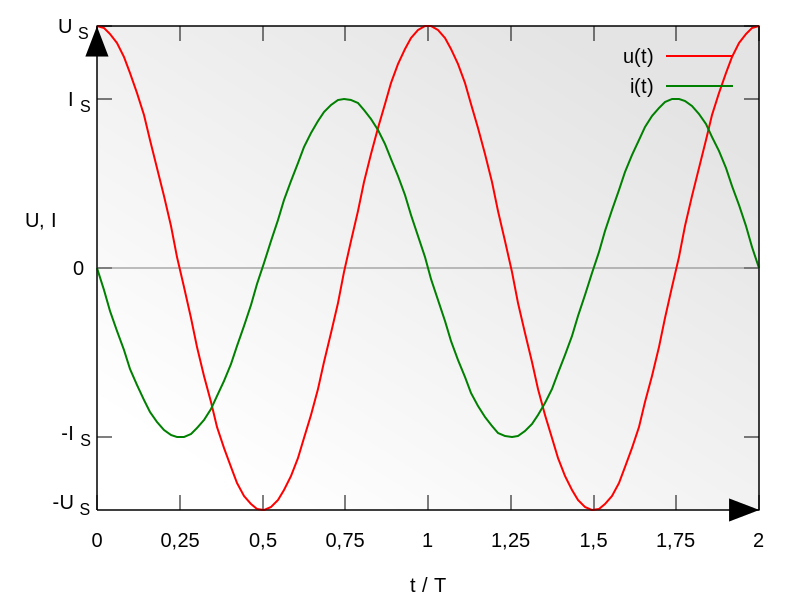
\includegraphics[width=1\textwidth]{a03/Sinus_Voltage_and_Current_of_a_Capacitor.png}
        \tiny \hyperlink{refs}{\cite{wc}}
    \end{center}
\end{frame}

\begin{frame}
\frametitle{Merksatz Kondensator}
\begin{center}
		\huge{Beim Kondensator - Eilt der Strom vor}
\end{center}
\end{frame}

\begin{frame}
    \frametitle{Wie verhält sich diese Schaltung}
	\begin{center}
        \includegraphics[width=.8\textwidth]{a03/Spulenstrom.png}
        \tiny \hyperlink{refs}{\cite{wc}}
    \end{center}
\end{frame}

\begin{frame}
	\frametitle{Spule}
\begin{minipage}{0.3\textwidth}
	\includegraphics[scale=0.13]{a03/Spulenstrom.png}
	\tiny \hyperlink{refs}{\cite{wc}}
\end{minipage}
\begin{minipage}{0.49\textwidth}
	\includegraphics[scale=0.35 ]{a03/Selbstinduktion-im-gleichstromkreis-zeitverlauf.png}
	\tiny \hyperlink{refs}{\cite{wc}}
\end{minipage}
\end{frame}

\begin{frame}
    \frametitle{Phasenverschiebung Spule}
	\begin{center}
        \includegraphics[width=1\textwidth]{a03/Phasenverschiebung_induktiv.png}
        \tiny \hyperlink{refs}{\cite{wc}}
    \end{center}
\end{frame}

\begin{frame}
\frametitle{Merksatz Spule}
\begin{center}
		\huge{Bei Induktivitäten, Ströme sich verspäten.}
\end{center}
\end{frame}

\begin{frame}
\frametitle{Merksatz Spule}
\begin{center}
		\huge{Wie verhalten sich Strom und Spannung beim Kondensator?}
\end{center}
\end{frame}

\begin{frame}
\frametitle{Merksatz Widerstand}
\begin{center}
		\huge{Beim reinen Ohmschen Widerstand gehn Strom und Spannung Hand in Hand}
\end{center}
\end{frame}

\section*{Komplexer Widerstand}

\begin{frame}
	\frametitle{Blindwiderstand}
\begin{minipage}{0.49\textwidth}
	\huge{Kondensator}\\
	\huge{$X_{C} = \frac{1}{\omega C}$}
\end{minipage}
\begin{minipage}{0.49\textwidth}
	\huge{Spule}\\
	\huge{$X_{L} = \omega L$}
\end{minipage}
\begin{center}
	\vspace{1cm}
Was war nochmal $\omega$? \\
\end{center}
\end{frame}

\begin{frame}
\frametitle{Komplexer Widerstand}
\begin{center}
		\includegraphics[width=.8\textwidth]{a03/Widerstand_Zeiger.png}
        \tiny \hyperlink{refs}{\cite{wc}}
Für den Gesamtwiderstand gilt\\
\huge{$Z = R + jX$}\\
\huge{$|Z| = \sqrt{R^2 + X^2}$}
\end{center}
\end{frame}
	
\begin{frame}
\frametitle{Elko Ersatzschaltbild}
\begin{center}
		\includegraphics[width=.8\textwidth]{a03/Elko-Ersatzschaltbild.png}
        \tiny \hyperlink{refs}{\cite{wc}}\\
        nach DIN EN 60384-1 vom Februar 2002 \\
        \huge{$R_{Leak}$} \normalsize Leckströme am Elko\\
        \huge{$R_{ESR}$} \normalsize ohmschen Verluste des Bauelementes\\
        \huge{$L_{ESL}$} \normalsize Induktivität des Bauelementes\\
        \huge{Verlustfaktor tang$\delta$} \normalsize Angabe in alten Datenblättern im Bezug auf ESR ($\omega C \cdot$ ESR $=$ tang$\delta$)
\end{center}
\end{frame}
	

\section*{Reihen und Parallelschaltung}

\begin{frame}
    \frametitle{Reihen und Parallelschaltung von Kondensatoren}
    \begin{center}
		\huge Wie war noch einmal die Formel für Kondensatoren in Reihen und Parallelschaltung?
    \end{center}
 \end{frame}
 
 \begin{frame}
    \frametitle{Parallelschaltung von Kondensatoren}	
 	\huge{$C_{ges} = C_{1} + C_{2} + C_{3} + C_{4} + C_{5}$} 
\end{frame}
    
\begin{frame}
    \frametitle{Reihenschaltung von Kondensatoren}
    \begin{center}
		\huge{$\frac{1}{C_{ges}} = \frac{1}{ C_{1}} + \frac{1}{C_{2}} + \frac{1}{C_{3}} + \frac{1}{C_{4}} + \frac{1}{C_{5}}$}\\
    \end{center}
\end{frame}

\begin{frame}
    \frametitle{Reihen und Parallelschaltung von Spulen}
    \begin{center}
		\huge Wie war noch einmal die Formel für die Spule in Reihen und Parallelschaltung von ?
    \end{center}
\end{frame}

\begin{frame}
    \frametitle{Reihen und Parallelschaltung von Spulen}
    
    $$L_{gesamt} = L_1 + L_2 + L_3 + ...$$\\
	$$\frac{1}{L_{gesamt}} = \frac{1}{L_1} + \frac{1}{L_2} + \frac{1}{L_3} + ...$$
\end{frame}

\section*{Induktivitäten mit Kern}

\begin{frame}
    \frametitle{Spule mit Kern}
    \begin{center}
		Für große Induktivitäten werden die Spulen um einen Kern gewickelt.\\
		Wichtiger Wert dafür ist der Kernfaktor\huge $A_{L}$ \normalsize(immer im Datenblatt)
	\huge	$$L = A_{L} N^2$$
    \end{center}
 \end{frame}
 
 \section*{Transformator}
\begin{frame}
    \frametitle{Transformator}
        \begin{center}
        \includegraphics[width=0.9\textwidth]{a03/trafo-Real.jpg}
        \footnote{\tiny \url{https://commons.wikimedia.org/wiki/File:Trafo_6.jpg}}
         \end{center}
\end{frame}

\begin{frame}
    \frametitle{Transformator}
    $$\text{\"u} = \frac{N_1}{N_2} = \frac{U_1}{U_2}$$
    	\vspace{1cm}
    $$P_1 = P_2$$
    $$U_{1} \cdot I_1 = U_{2} \cdot I_2 $$
  \huge  $$\frac{U_1}{U_2} = \frac{I_2}{I_1}$$
\end{frame}

\begin{frame}
    \frametitle{Widerstandsanpassung}
   \huge  $$\text{\"u} = \frac{N_2}{N_1} = \sqrt{\frac{R_1}{R_2}}$$
    	\vspace{1cm}
    \normalsize Wird benötigt z.B. wenn der Fußpunktwiderstand einer Antenne bei $200 \Omega$ liegt aber mit einem $50\Omega$ Coaxkabel gespeist werden soll.
\end{frame}

\section*{Balun}

\begin{frame}
    \frametitle{Balun Theorie}
	\begin{center}
        \includegraphics[width=0.8\textwidth]{a03/Cdbalun2.png}
                \tiny \hyperlink{refs}{\cite{wc}}
    \end{center}
\end{frame}

\begin{frame}
    \frametitle{Balun Real}
	\begin{center}
        \includegraphics[width=0.9\textwidth]{a03/balun-Real.jpg}
                \tiny \hyperlink{refs}{\cite{wc}}
    \end{center}
\end{frame}


\renewcommand{\refname}{Referenzen}

\hypertarget{refs}{}
\textcolor{white}{} \\ %\vspace{} geht nicht
\Large Referenzen/Links
\footnotesize

\begin{thebibliography}{}
    \bibitem{dj4uf} Moltrecht A 03: \\
                    \url{http://www.darc.de/referate/ajw/ausbildung/darc-online-lehrgang/technik-klasse-a/technik-a03/}

    \bibitem{wc}    Wikimedia Commons: \\
                    \url{https://commons.wikimedia.org/wiki/File:Sinus_Voltage_and_Current_of_a_Capacitor.svg}\\
                    \url{https://commons.wikimedia.org/wiki/File:Selbsti.gif}\\
                    \url{https://commons.wikimedia.org/wiki/File:Selbstinduktion-im-gleichstromkreis-zeitverlauf.svg}\\
                    \url{http://commons.wikimedia.org/wiki/File:Capacitors_(7189597135).jpg}\\
                    \url{https://commons.wikimedia.org/wiki/File:Phasenverschiebung_induktiv.svg}\\
                    \url{https://commons.wikimedia.org/wiki/File:Widerstand_Zeiger.svg}\\
                    \url{https://commons.wikimedia.org/wiki/File:Elko-Ersatzschaltbild-Wiki-07-02-08.svg}\\
                    \url{https://commons.wikimedia.org/wiki/File:T200A2.jpg}\\
                    \url{https://commons.wikimedia.org/wiki/File:Cdbalun2.svg}\\
\end{thebibliography} 

% Hier könnte noch eine Kontaktfolie stehen

\end{document}

